%!TEX root = ../Pflichtenheft.tex

\chapter{Instructions}\label{chap:zielbestimmung}
Dear user,\\
we are delighted that you use our Framework for Neo4j. So that everything runs accordingly you only need Neo4j, Maven and Java for our functions and it runs on every normal operating system.
If you have any questions, please do not hesitate to contact us on our \glqq Git Repository\grqq{}.

\section{Required-Software}\label{sec:neededsoftware}
You need for this Framework definitely:
\begin{itemize}
	\item The Software for Neo4j \footnote{\url{https://neo4j.com/download/other-releases/\#releases}} is very important; it has to be installed otherwise you can't run the framework.
	\item On your device should be installed the newest version from Java\footnote{\url{https://java.com/de/download/}} and the needed root-settings are set.
	\item Also your device need Maven\footnote{\url{https://maven.apache.org/download.cgi}}, this is important for the \glqq Neo4j - Procedures \grqq{}.
\end{itemize}
For a better programming success we recommend to take an IDE. For the instruction we take IntelliJ IDEA\footnote{\url{https://www.jetbrains.com/idea/download}}. If you really need this instruction, you should download IntelliJ IDEA and you can install the Framework easy step by step (See point \ref{sec:stepByStepManual} Step by Step Manual).

\newpage

\section {First use guidance for experienced users} \label{sec:beforeFirstUse}
\begin{itemize}
	\item The required Software should be installed on your computer and so you can be sure that everything works right.
	\item Please start the Neo4j - Software and create a new Database. 
	\item Please create in this Folder (neo4j/default.graphdb) a new Folder with the name \glqq plugins\grqq{}. You need this for your \glqq  Neo4j - Procedures\grqq{}.
	\item Now you need our Framework. You can clone our \glqq Git Repository\footnote{\url{https://github.com/vonunwerth/neo4j.git}} \grqq{}. If you don't now how you clone the \glqq Git Repository\grqq{} please read the Step by Step Manual.
	\item Furthermore you must download the \glqq Maven Dependencies\grqq{} ++++ WIE? +++. If you use an IDE the IDE can do this for you.
	\item At the package \glqq matcher\grqq{} you can create a new Java class where you write your algorithm.
	\item Where and what needs to be changed at this class, so that \glqq Neo4j - procedures\grqq{} can work properly we explain at chapter \ref{sec:startProgramming} \glqq Start\grqq{} coding. 
\end{itemize}

\section{Step by Step for beginners}\label{sec:stepByStepManual}
This Step by Step is created for using the software \glqq ItelliJ IDEA\grqq{}.
\begin{itemize}
	\item The requested Software should be installed on your computer and be sure that everything works right.
	\item Please start the Neo4j - Software and create a new database. You create it step by step with Neo4j. The only important thing is to know where the storage is. (The Folder is called by default neo4j/default.graphdb). \\(Nice to know for login: by default is user:neo4j, password:neo4j)
	\item Please create in this Folder (neo4j/default.graphdb) a new Folder with the name \glqq plugins\grqq{}. You need this for your \glqq  Neo4j - Procedures\grqq{}.
	\newpage
	\item After downloading the Software \glqq ItelliJ IDEA\grqq{} opens and ready for use.The following windows opens. \\
	\begin{center}
		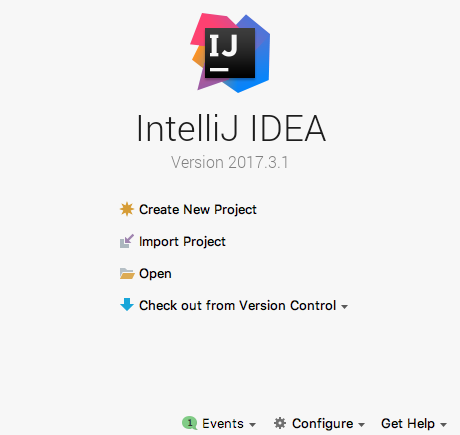
\includegraphics[width=4.2cm]{common/IntelliJstart.png}\setlength{\unitlength}{1mm}
	\end{center}

	\item You click on \glqq Check out from Version Control\grqq{} and a window with the name \glqq Clone Repository\grqq{} will be open. \\
	\textbf{Git Repository URL:} https://github.com/vonunwerth/neo4j.git \\
	\textbf{Parent Directory:} It's your memory location \\
	\textbf{Directory Name:} For example Neo4j (You can choose what ever you want.)\\
	\\
	Now you are downloading our Repository to your computer.
	
	\item The Folder with our \glqq Git Repository\grqq{} is displayed at the \glqq IntelliJ\grqq{} window, but you only see \glqq readme\grqq{}and other data but not the Java files. \\
	If you want see the Java files, open the Maven Tab on the right side. Click on the tab and on the circle on the left corner. You will be ask, if you want to \glqq import Maven Projects\grqq{} - click \glqq yes\grqq{}. The \glqq Maven Dependencies\grqq{} are now downloaded, this needs a while.
	\begin{center}
		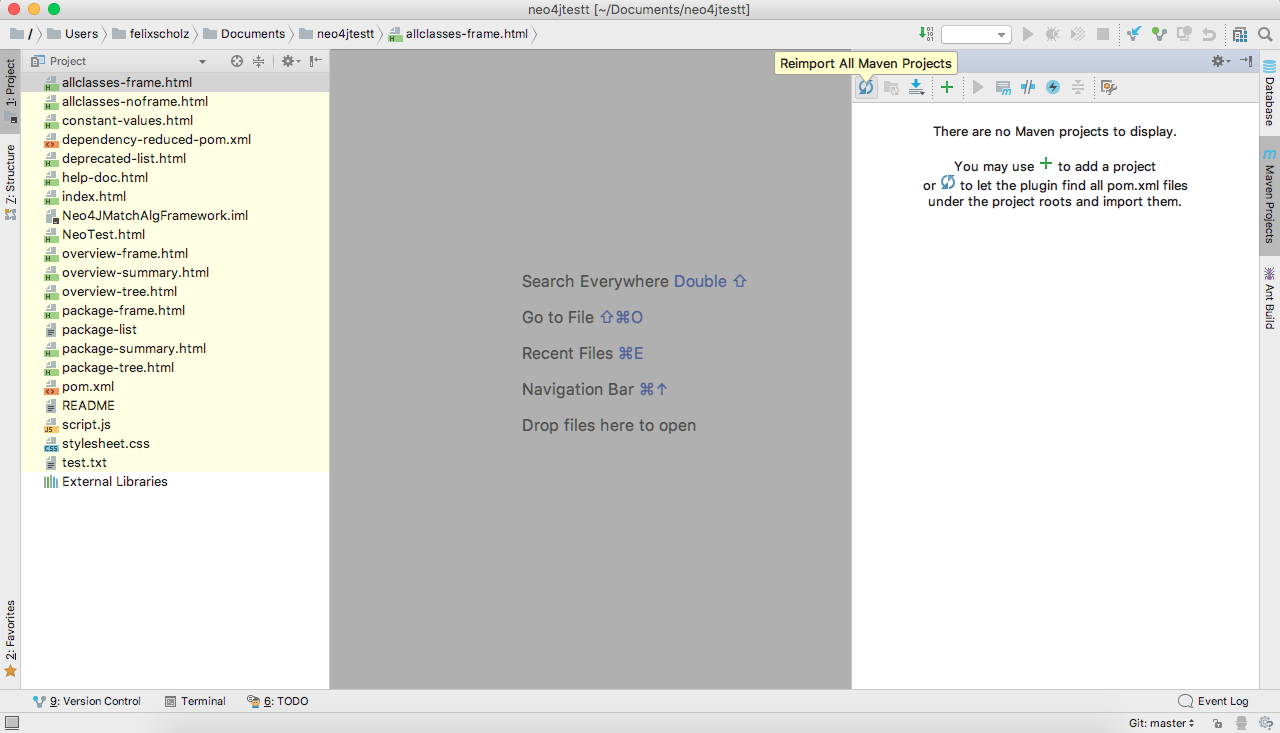
\includegraphics[width=14.5cm]{common/MavenImport.png}\setlength{\unitlength}{1mm}
	\end{center}
	\item All Folder become visible. Open the src/main/java folder.
	\item At the \glqq package matcher\grqq{} you can create a new Java file where you write your algorithm.
\end{itemize}

\section{Start coding}\label{sec:startProgramming}
On your Computer is the \glqq Git Repository\grqq{} and the IDE doesn't show any errors? At this point you can start.
\begin{itemize}
	\item The new class in the \glqq matcher - package \grqq{} must be abstract.
	\item You have to write a constructor at your class. The constructor (The name must be the same like the classname(the definition for a constructor)). The following structure must be used: \\
	\lstset{language=Java}
	\begin{lstlisting}
	public ???(GraphDatabaseService db, Graph graph) {
		this.db = db;
		this.graph = graph;
	}
	\end{lstlisting}
	%\begin{center}
	%	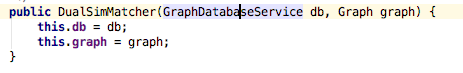
\includegraphics[width=10.5cm]{common/MatcherConstrutor.png}\setlength{\unitlength}{1mm}
	%\end{center}
	\item The next step is to implement the \glqq matchingAlgorithm\grqq{}. This method is for your algorithm and there you can write what ever you want. \\
	\lstset{language=Java}
	\begin{lstlisting} 
	 @Override
	public Map<Integer, List<Node>> matchingAlgorithm() {
	\end{lstlisting} 
	If you need other help you find a lot helpful methods in the class \glqq matcher \grqq{} Check our API.
	\item After finishing your algorithm, you have to do two more things: \\ 
	\begin{enumerate}
		\item Change the name of the algorithm object.(GraphProcdures.java Line 56) \\
		\item Change the procedures name - if you like - it's no must.!(GraphProcdures.java \\
		Line 39) \\
	See the red lines.
	\end{enumerate}
	\begin{center}
		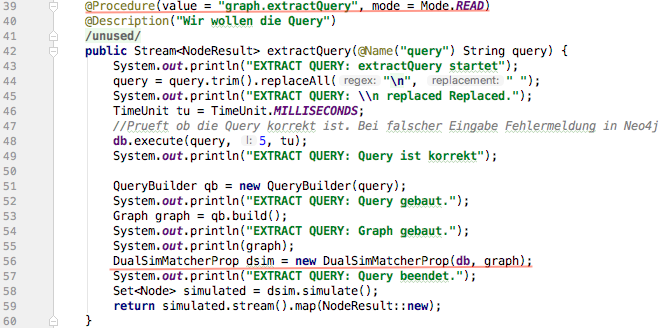
\includegraphics[width=9.0cm]{common/ChangeProcedures.png}\setlength{\unitlength}{1mm}
	\end{center}
\end{itemize}

\section{After coding}\label{sec:afterProgramming}
After you write your algorithm in your new class at the Java package matcher, you have to create the \glqq jar \grqq{} for the database.
\begin{itemize}
	\item Before you create the jar, you can test the code. Please use the API and the test package. For testing please start the class \glqq ProceduresTest.java\grqq{}.
	\item Open the Maven tab in \glqq ItelliJ \grqq{} and open the point \glqq Neo4JMatchAlgFramework\grqq{}. The next folder you need is the \glqq Lifecycle\grqq{} folder, there you click \glqq clean\grqq{} and after this runs you click on \glqq package\grqq{}.
	\item The Maven action is finishing? Then you go in your explorer and search the folder where you clone the \glqq Git Repository\grqq{}. There is a new folder named target. Open this \glqq folder\grqq{} and copy the \glqq original-Neo4JMatchAlgFramework-1.0.jar\grqq{}. \\
	(The other one is for testing and it is not important. It wouldn't work.)
	\item Please go to your Neo4j database from the first steps.(see step by step manual) You must paste the \glqq original-Neo4JMatchAlgFramework-1.0.jar\grqq{} in the created \glqq plugins\grqq{} Folder.
	\item After you do this the Neo4j database knew your algorithm. If you are ready open the database with the Neo4j software.
\end{itemize}

\section{Work with Neo4j}\label{sec:takeneo4j}
The very last thing is checking your algorithm is faster or better then everything else.
For this you definitely need the following
\newpage
\begin{itemize}
	\item You want to use your procedures? Then take the CALL-Statement.\\
	For example:
	\begin{lstlisting}
	CALL graph.extractQuery(
	"MATCH (m:Movie)<-[:DIRECTED]-(p:Person) 
	RETURN m,p")
	\end{lstlisting}
	\item You want to take your procedures and would like to search with an other query on this result? Then take the CALL statement and the YIELD statement. \\
	For example:
	
	\begin{lstlisting}
	CALL graph.extractQuery(
	"MATCH (m:Movie)<-[:DIRECTED]-(p:Person)
	RETURN m,p") 
	yield node MATCH (m:Movie)<-[:DIRECTED]-(p:Person)
	RETURN m,p
	\end{lstlisting}
\end{itemize}
At this point you know everything we know - So have fun and develop new good algorithms.

